\title{Raport projektu}
\author{
	Julia Czerniecka 262208
    \and
	Wiktoria Gałdusińska 262209
	\and
	Jerzy Grunwald 262237
	\and
    Maciej Kosierb 262239 
    \and
    Krzysztof Mizgała 262839
}
\date{\today}

\documentclass[12pt]{article}
\usepackage[hidelinks]{hyperref}
\usepackage{polski}
\usepackage[utf8]{inputenc}
\usepackage{pgf-umlcd}
\usepackage{listings}
\usepackage{graphicx}
\usepackage{float}
\usepackage{xcolor}
\usepackage{xparse}
\usepackage{verbatim}
\usepackage{geometry}
\geometry{a4paper, left=25mm, top=25mm}
\setlength{\parindent}{0pt}

\NewDocumentCommand{\codeword}{v}{
    \texttt{\textcolor{blue}{#1}}
}

\begin{document}
    \maketitle
    \tableofcontents
    \newpage

    \section{Wstęp}\label{sec:wstep}
  
Jeżeli podczas pracy w~\TeX-u napotkamy problem, dobrym instynktem jest wyszukanie go w~internecie. W~większości przypadków jesteśmy w~stanie znaleźć odpowiedź na nasze pytanie m.in. na forach, takich jak \TeX~Stack Exchange. Jeśli nie uda nam się znaleźć rozwiązania napotkanego problemu, możemy również zamieścić pytanie na forum, tym samym licząc na pomoc ponad $260$ tysięcy użytkowników. Jeśli jednak osoby zadające pytania nie otrzymają oczekiwanych odpowiedzi, strony te nie będą użyteczne. Na Stack Exchange, jedynym znakiem pokazującym, że osoba zadająca pytanie uzyskała pożądaną odpowiedź, jest akceptacja odpowiedzi. W~tym projekcie badamy pytania i~zaakceptowane odpowiedzi z~forum \TeX~Stack Exchange, w~celu zrozumienia, jakie czynniki wpływają na akceptację odpowiedzi.

	\section{Opis danych}\label{sec:opis-danych}

	Skorzystaliśmy z~dostępnych zrzutów danych Stack Exchange, dotyczących forum \TeX-a, udostępnionych przez \underline{\href{https://archive.org/details/stackexchange}{archive.org}}. Dane składają się z~trzech istotnych dla nas tabel:
	\begin{enumerate}
		\item \verb|posts|, zawierającej wszystkie nieusunięte posty; kolumny, z~których korzystamy to:
		\begin{itemize}
			\item PostTypeId -- typ wpisu (1 -- pytanie);
			\item AcceptedAnswerId -- ID zaakceptowanej odpowiedzi (NULL -- brak zaakceptowanej odpowiedzi); 
			\item CreationDate -- data zadania pytania;
			\item Title -- tytuł pytania;
			\item Body -- treść pytania;
			\item OwnerUserId -- ID użytkownika zadającego pytanie;
			\item Tags -- lista tagów pytania;
		\end{itemize}
		\item \verb|users|, która posiada informacje na temat użytkowników forum; kolumny, z~których korzystamy to:
		\begin{itemize}
			\item Id -- ID użytkownika;
			\item CreationDate -- data założenia konta na forum;
			\item Reputation -- reputacja użytkownika (podana w~postaci liczby całkowitej);
			\item Views -- liczba wyświetleń profilu;
			\item UpVotes -- liczba pozytywnie ocenionych postów przez użytkownika;
			\item DownVotes -- liczba negatywnie ocenionych postów przez użytkownika;
		\end{itemize}
		\item \verb|tags| z~informacjami na temat tagów; kolumny, z~których korzystamy to:
		\begin{itemize}
			\item TagName -- nazwa tagu;
			\item Count -- liczba pytań z~danym tagiem.
		\end{itemize}
	\end{enumerate}
	
	\section{Metodyka}\label{sec:metodyka}
	Do efektywnego przetwarzania ogromnej ilości danych zastosowaliśmy popularne środowisko obsługujące Big Data, jakim jest Apache Spark. Umożliwił on równoległe i~rozproszone przetwarzanie danych.
	
	\vspace{0.25cm}
	
	Przeprowadzono zaawansowane przetwarzanie cech (ang. feature engineering) na danych wejściowych, aby lepiej odzwierciedlić istotne aspekty pytania, takie jak:
	\begin{itemize}
		\item TitleLength -- długość tytułu pytania (liczba słów);
		\item BodyLength -- długość treści pytania (liczba słów);
		\item NumberOfTags -- liczba tagów;
		\item TagsCountMax -- popularność tagów (liczba pytań, w~których wystąpił najpopularniejszy z~tagów);
		\item informacje o~pytającym:
		\begin{itemize}
			\item OwnerReputation -- reputacja;
			\item OwnerViews -- wyświetlenia profilu;
			\item OwnerUpVotes, OwnerDownVotes -- liczba pozytywnie i~negatywnie ocenionych postów przez użytkownika;
			\item OwnerExperience -- doświadczenie w~momencie zadawania pytania (liczba dni od daty założenia konta na forum do momentu zadania pytania);
		\end{itemize}
		\item Accepted -- stan akceptacji odpowiedzi (czy pytania posiada zaakceptowaną odpowiedź).
	\end{itemize}
	Rozważamy jedynie wyżej wymienione cechy, ponieważ są to wszystkie istotne informacje dostępne w~momencie zadania pytania.
	
	\vspace{0.25cm}
	
	Tworzymy tabelę pomocniczą \verb|questions|, która zawiera powyższe cechy dla każdego pytania w~tabeli \verb|posts|.
	
	\vspace{0.25cm}
	
	Implementujemy cztery modele predykcyjne, mające na celu przewidzenie, czy pytanie otrzyma zaakceptowaną odpowiedź, czy też nie. Do uczącej części danych dopasowano następujące modele:
	\begin{itemize}
		\item model regresji logistycznej;
		\item model lasów losowych;
		\item gradient boosting;
		\item model sieci neuronowych.
	\end{itemize}
	
    \section{Analiza opisowa danych}\label{sec:analiza-opisowa-danych}
	Tabela \verb|posts| zawiera $584\,821$ rekordów, z~czego $255\,804$ stanowią pytania. Okazuje się, że $60,13\%$ pytań ma zaakceptowaną odpowiedź oraz $47,16\%$ spośród wszystkich odpowiedzi jest zaakceptowanych. Wysoki wskaźnik akceptacji może sugerować, że społeczność skutecznie zapewnia pomocne odpowiedzi.
	
	\begin{figure}[H]
		\centering
		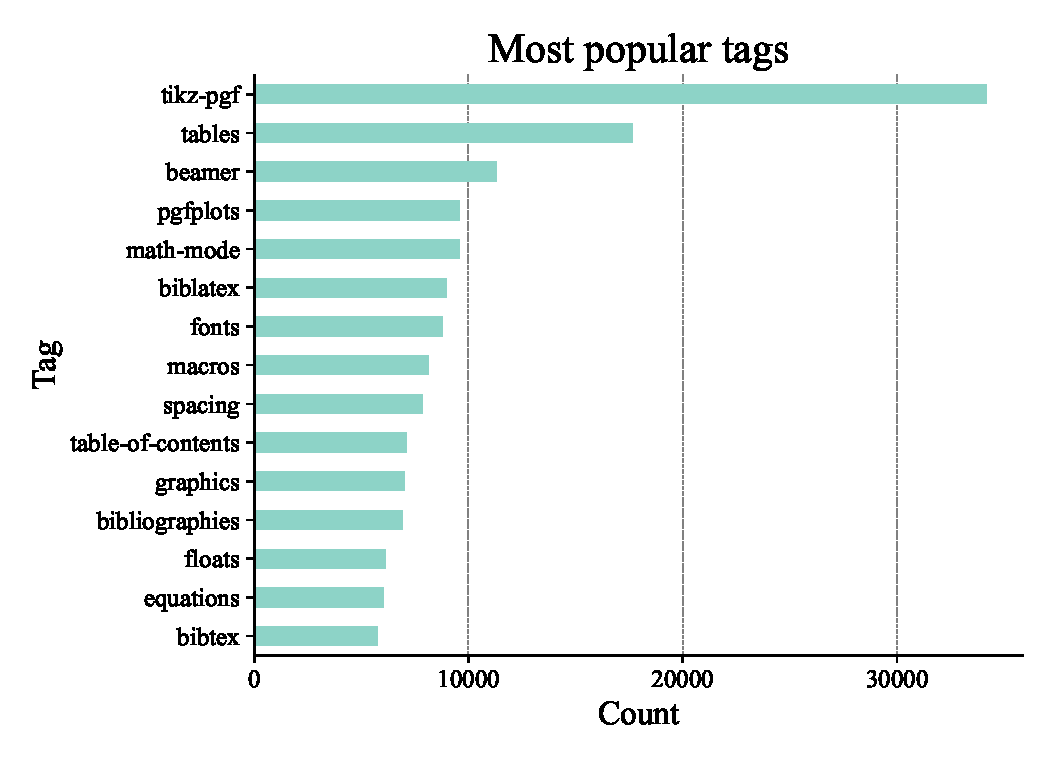
\includegraphics[width=0.7\textwidth]{tags_popularity}
		\caption{Najpopularniejsze tagi}
		\label{fig:most-popular-tags}
	\end{figure}
	Wykres ten przedstawia najczęściej wykorzystywane przez użytkowników forum tagi. Najbardziej popularnym tagiem jest ,,tikz-pgf", co wskazuje, że użytkownicy często zadają pytania związane z~TikZ - pakietem \LaTeX~umożliwiającym programowe tworzenie grafiki. 
	
	\begin{figure}[H]
		\centering
		\includegraphics[width=0.7\textwidth]{tags_top}
		\caption{Najwyższe prawdopodobieństwa uzyskania zaakceptowanej odpowiedzi dla tagów posiadających ponad $1\,000$ pytań}
		\label{fig:najwyzsze-prawdopodobienstwa-uzyskania-odpowiedzi-tagi}
	\end{figure}
	\begin{figure}[H]
		\centering
		\includegraphics[width=0.7\textwidth]{tags_bottom}
		\caption{Najniższe prawdopodobieństwa uzyskania zaakceptowanej odpowiedzi dla tagów posiadających ponad $1\,000$ pytań}
		\label{fig:najnizsze-prawdopodobienstwa-uzyskania-odpowiedzi-tagi}
	\end{figure}
	Wykresy te wskazują na to, że prawdopodobieństwo uzyskania zaakceptowanej odpowiedzi istotnie zależy od wykorzystanych tagów. Pytania z~tagami  ,,expansion" i~,,expl3" mają wyższe prawdopodobieństwo zaakceptowania odpowiedzi, co może oznaczać, że społeczność jest najbardziej aktywna wokół tematów z~nimi powiązanych lub że te tematy są łatwiejsze do rozwiązania. Tagi ,,texmaker" i~,,miktex" posiadają najniższe prawdopodobieństwo uzyskania zaakceptowanej odpowiedzi, co może oznaczać, że problemy, z~którymi zmagają się użytkownicy w~tej kategorii są wymagające i~społeczność nie potrafi ich rozwiązać.
	
	\begin{figure}[H]
		\centering
		\includegraphics[width=0.7\textwidth]{tags_number}
		\caption{Prawdopodobieństwa uzyskania zaakceptowanej odpowiedzi w~zależności od liczby tagów}
		\label{fig:prawdopodobienstwa-uzyskania-odpowiedzi-liczba-tagow}
	\end{figure}
	Powyższy wykres słupkowy pokazuje, że pytania zawierające od dwóch do pięciu tagów mają nieco większe szanse na otrzymanie zaakceptowanej odpowiedzi w~porównaniu do tych z~jednym tagiem. Może to wskazywać, że liczba tagów nie wpływa w~dużym stopniu na prawdopodobieństwo uzyskania zaakceptowanej odpowiedzi.
	
	\begin{figure}[H]
		\centering
		\includegraphics[width=0.7\textwidth]{user_reputation}
		\caption{Prawdopodobieństwa uzyskania zaakceptowanej odpowiedzi w~zależności od reputacji zadającego pytanie}
		\label{fig:prawdopodobienstwa-uzyskania-odpowiedzi-reputacja}
	\end{figure}
	Wykres pokazuje pozytywną korelację między reputacją pytającego a~prawdopodobieństwem zaakceptowania odpowiedzi na jego pytanie. W~przypadku użytkowników z~najwyższą reputacją, prawdopodobieństwo otrzymania odpowiedzi, która zostanie zaakceptowana jest największe. Może to wynikać z~większego doświadczenia w~formułowaniu pytań na forum.
	
	\begin{figure}[H]
		\centering
		\includegraphics[width=0.7\textwidth]{question_creation_date}
		\caption{Prawdopodobieństwa uzyskania zaakceptowanej odpowiedzi w~zależności od daty publikacji pytania}
		\label{fig:prawdopodobienstwa-uzyskania-odpowiedzi-data}
	\end{figure}
	Wykres wskazuje, że prawdopodobieństwo otrzymania zaakceptowanej odpowiedzi na pytanie wzrasta wraz z~czasem. Im starsze pytanie, tym większa szansa, że posiada ono zaakceptowaną odpowiedź.
	
	\begin{figure}[H]
		\centering
		\includegraphics[width=0.7\textwidth]{user_experience}
		\caption{Prawdopodobieństwa uzyskania zaakceptowanej odpowiedzi ze względu na długość członkostwa pytającego}
		\label{fig:prawdopodobienstwa-uzyskania-odpowiedzi-czlonkostwo}
	\end{figure}
	Powyższy wykres pozwala wysnuć wniosek, że prawdopodobieństwo pozostaje stosunkowo stabilne, niezależnie od tego, jak długo użytkownik jest członkiem forum, co sugeruje, że długość członkostwa nie wpływa znacząco na szanse otrzymania zaakceptowanej odpowiedzi.
	
	\begin{figure}[H]
		\centering
		\includegraphics[width=0.7\textwidth]{user_upvotes}
		\caption{Prawdopodobieństwa uzyskania zaakceptowanej odpowiedzi ze względu na liczbę pozytywnie ocenionych postów przez pytającego}
		\label{fig:prawdopodobienstwa-uzyskania-odpowiedzi-upvotes}
	\end{figure}
	Na podstawie wykresu można stwierdzić, że istnieje znacząca zależność prawdopodobieństwa uzyskania zaakceptowanej odpowiedzi od liczby pozytywnie ocenionych postów przez pytającego.
	
	\begin{figure}[H]
		\centering
		\includegraphics[width=0.7\textwidth]{user_downvotes}
		\caption{Prawdopodobieństwa uzyskania zaakceptowanej odpowiedzi ze względu na liczbę negatywnie ocenionych postów przez pytającego}
		\label{fig:prawdopodobienstwa-uzyskania-odpowiedzi-downvotes}
	\end{figure}
	Warto wspomnieć, że użytkownicy mają możliwość ocenienia postów w~negatywny sposób tylko wtedy, gdy przekroczą pewien próg reputacji. Ponadto, wystawiając negatywną opinię, tracą punkty reputacji. Z~tego względu, użytkownicy rzadko decydują się na przyznawanie negatywnych ocen. Można spekulować, że jedynie doświadczeni i~najbardziej aktywni członkowie forum wystawiają negatywne oceny, a~zatem cecha OwnerDownVotes może być skorelowana z~cechą OwnerReputation.
	
	\section{Analiza istotności cech}\label{sec:analiza-istotnosci-cech}
	Tworzymy klasyfikator drzew losowych oparty o~aspekty pytania opisane w~sekcji \ref{sec:metodyka}. Dla wybranego ziarna generatora, otrzymujemy następujące współczynniki istotności cech (w przybliżeniu do dwóch miejsc po przecinku):
	\begin{itemize}
		\item OwnerUpVotes: $46,25\%$;
		\item OwnerReputation: $31,06\%$;
		\item OwnerViews: $11,02\%$;
		\item OwnerExperience: $6,44\%$;
		\item TagsCountMax: $2,46\%$;
		\item OwnerDownVotes: $2,09\%$;
		\item BodyLength: $0,48\%$;
		\item TitleLength: $0,10\%$;
		\item NumberOfTags: $0,19\%$.
	\end{itemize}
	Można zaobserwować, że wnioski uzyskane w~sekcji \ref{sec:analiza-opisowa-danych} są istotnie powiązane z~powyższymi wynikami.
	
	\vspace{0.25cm}
	
	Aby uniknąć przeparametryzowania modeli, w~dalszych analizach będziemy rozważać jedynie te cechy, których istotność wynosi przynajmniej $1\%$.
	
	\section{Wybór najlepszego modelu}\label{sec:wybor-najlepszego-modelu}
	Posiadając informacje na temat istotności cech możemy przystąpić do konstrukcji modeli. Dzielimy dane na część uczącą i~testową w~stosunku $80/20$. Dla danych uczących dopasowujemy cztery modele. Następnie wyznaczamy predykcje uzyskania zaakceptowanej odpowiedzi dla danych ze zbioru testowego i~badamy jakość modeli w~oparciu o: 
	\begin{itemize}
		\item dokładność dopasowania (Accuracy); 
		\item wskaźnika Bookmaker Informedness (BM);
		\item współczynnik korelacji Matthewsa (MCC). 
	\end{itemize}

	\subsection{Wykorzystywane miary dokładności}\label{subsec:miary-dokladnosci}
	
	\subsubsection{Dokładność (Accuracy)}
	Jest to miara statystyczna wykorzystywana w~kontekście klasyfikacji w~uczeniu maszynowym i~statystyce do mierzenia stopnia zgodności między przewidywaniami modelu a~rzeczywistymi wartościami. Określa ona stosunek liczby poprawnych przewidywań do całkowitej liczby przypadków w~zbiorze danych i~przedstawia się wzorem 
	\[\mathrm{Dokładność} = \frac{\mathrm{Dobrze~dopasowane~przypadki}}{\mathrm{Liczność~populacji}}.\] 
	Dużą zaletą tej miary jest jej prostota i~łatwość w~interpretacji. Pomimo tego, ze względu na brak uwzględnienia nierównomiernego rozkładu klas, wysoka dokładność może być myląca, gdy jedna klasa jest znacznie liczniejsza niż pozostałe. Model może osiągnąć wysoką dokładność, zawsze przewidując dominującą klasę, co nie świadczy o~jego rzeczywistej skuteczności. Z~tego względu, do oceny modeli wykorzystamy również inne miary.
	
	\subsubsection{Bookmaker Informedness (BM)}
	Jest to miara oceniająca skuteczność klasyfikatora binarnego, która mierzy zdolność klasyfikatora do unikania fałszywych klasyfikacji, łącząc czułość i~specyficzność w~jedną metrykę. Wartość BM wynosi od $0$ (brak wartości informacyjnej) do $1$ (doskonała informacyjność), gdzie wyższe wartości wskazują na lepszą wydajność klasyfikatora. Miara ta przedstawia się wzorem
	\[BM = \mathrm{Czułość} + \mathrm{Swoistość} - 1.\] 
	Zaletami tej miary są prostota interpretacji oraz zdolność do oceny ogólnej skuteczności klasyfikatora w~unikaniu fałszywych klasyfikacji. Pomimo tego jest mniej przydatna w~niezbalansowanych zbiorach danych, gdzie liczba przypadków w~klasach jest istotnie różna.
	
	\subsubsection{Współczynnik korelacji Matthewsa (MCC)}
	Jest to miara służąca do oceny jakości klasyfikacji binarnych, uwzględniająca wszystkie cztery części macierzy pomyłek: prawdziwie pozytywne, fałszywie pozytywne, prawdziwie negatywne i~fałszywie negatywne przypadki. Oferuje zbilansowaną ocenę klasyfikatorów, szczególnie w~niezbalansowanych zbiorach danych. MCC przyjmuje wartości od $-1$ do $1$, gdzie $1$ oznacza dobre dopasowanie, $0$ na poziomie klasyfikatora losowego, a~$-1$ oznacza całkowite niedopasowanie. Miara ta przedstawia się wzorem
	\[MCC = \frac{(TP \cdot TN) - (FP \cdot FN)}{\sqrt{(TP + FP)(TP + FN)(TN + FP)(TN + FN)}},\] 
	gdzie
	\begin{itemize}
		\item $TP$ - liczba prawdziwie pozytywnych wyników,
		\item $TN$ - liczba prawdziwie negatywnych wyników,
		\item $FP$ - liczba fałszywie pozytywnych wyników,
		\item $FN$ - liczba fałszywie negatywnych wyników.
	\end{itemize}
	
	\subsection{Model regresji logistycznej}\label{subsec:model-regresji-logistycznej}
	Model regresji logistycznej to matematyczny model służący do przewidywania prawdopodobieństwa przynależności obserwacji do jednej z~dwóch klas. Regresja logistyczna używa funkcji logistycznej do przekształcania wyników regresji liniowej na przedział $(0,1)$, co interpretowane jest jako prawdopodobieństwo.
	
	\vspace{0.25cm}
	
	Dopasowujemy model regresji logistycznej przyjmując maksymalną liczbę iteracji równą $100$.
	
	\subsection{Model lasów losowych}\label{subsec:model-lasów-losowych}
	Model lasów losowych to model zespołowy, który łączy wiele drzew decyzyjnych, a~następnie agreguje wyniki. Każde drzewo w~lesie losowym jest trenowane na innym podzbiorze danych, a~także losowo wybiera podzbiór cech do rozważania podczas węzłów. 
	
	\vspace{0.25cm}
	
	Dopasowujemy model lasów losowych przyjmując liczbę drzew równą $100$.
	
	\subsection{Gradient boosting}\label{subsec:gradient-boosting}
	Ogólna idea boostingu polega na trenowaniu modeli iteracyjnie, a~każdy nowy model jest dostosowywany do błędów poprzedniego.
	
	\vspace{0.25cm}
	
	Dopasowujemy model gradient boosting przyjmując maksymalną liczbę iteracji równą $100$.
	
	\subsection{Model sieci neuronowych}\label{subsec:model-sieci-neuronowych}
	Model sieci neuronowych to system obliczeniowy składający się z~warstw neuronów, z~których każdy jest połączony z~wieloma innymi neuronami, reprezentowanymi przez funkcje matematyczne. Model uczy się rozpoznawania wzorców, dokonywania klasyfikacji i~przewidywania wyników.
	
	\vspace{0.25cm}
	
	Warstwa wejściowa przyjmuje dane wejściowe, które mają $6$ cech. Mamy dwie warstwy ukryte oraz jedną warstwę wyjściową. Pierwsza warstwa ukryta ma $10$ neuronów, a~druga $8$. Warstwa wyjściowa ma $2$ neurony, ponieważ cecha Accepted jest typu binarnego. Parametry te zostały dobrane na bazie wielokrotnej walidacji.
	
	\subsection{Zestawienie dokładności dopasowania}\label{subsec:zestawienie-dopasowania-modeli}
	
	\begin{table}[H]
		\centering
		\begin{tabular}{c|cccc}
			\hline\hline
			       Model         & Accuracy &   BM  &  MCC   &  \\\hline
			Regresja logistyczna & 60,06\% &   ---  &   0    &  \\
			    Lasy losowe      & 70,27\% & 0,4232 & 0,3603 &  \\
			 Gradient boosting   & 70,92\% & 0,4243 & 0,3747 &  \\
			  Sieci neuronowe    & 66,38\% & 0,2980 & 0,2706 &  \\\hline
		\end{tabular}
		\caption{Tabela dokładności dopasowania modeli dla trzech wybranych miar w~zaokrągleniu}
		\label{tab:dokladnosc}
	\end{table}
	
	Miara BM przyjmuje dla regresji liniowej wartość nieokreśloną, ponieważ przy wyznaczaniu czułości dzielimy przez zero.
	Podobnie w~przypadku obliczania MCC dochodzi do dzielenia przez zero, jednakże w~tej sytuacji przypisanie wartości zero jest uzasadnione.
	Pełny dowód można znaleźć w
	\underline{\href{https://biodatamining.biomedcentral.com/articles/10.1186/s13040-021-00244-z}{artykule}}.
	
	\section{Podsumowanie}
	Interpretując wyniki w~tabeli \ref{tab:dokladnosc} zauważamy, że   gradient boosting wykazuje najlepszą ogólną wydajność wśród analizowanych modeli, zarówno pod względem dokładności, jak i~obu zastosowanych miar korelacji. Lasy losowe również prezentują się dobrze, będąc blisko wartości gradient boosting. Sieci neuronowe, choć lepsze od regresji logistycznej pod względem dokładności, nie osiągają tak dobrych wyników jak dwa wcześniej wspomniane modele w~kategoriach BM i~MCC. Regresja logistyczna ma najniższą dokładność i~MCC równy $0$, co sugeruje jej ograniczoną użyteczność w~porównaniu z~innymi modelami w~tym zestawieniu.
	
	\section{Lista plików}\label{sec:lista-plikow}
	Spis plików wchodzących w~skład projektu:
	\begin{itemize}
		\item folder tex.stackexchange.com -- tabele zawierające analizowane dane;
		\item statistics.ipynb -- analiza opisowa danych;
		\item features.ipynb -- analiza istotności cech;
		\item analysis.ipynb -- ocena dokładności modeli predykcyjnych;
		\item requirements.txt -- spis wykorzystywanych bibliotek;
		\item README.md -- informacje potrzebne do inicjalizacji analiz.
	\end{itemize}
	
\end{document}
